\documentclass[a4paper,12pt,spanish,final]{epsc_tfc_pfc}

%-----------
% Preamble:
%-----------

\usepackage[spanish,english]{babel}
\usepackage[utf8]{inputenc}
\usepackage{amssymb,amsmath,amsfonts}
\usepackage{array}
\usepackage{listings}
\usepackage{color}
\usepackage{eurosym}

%---------------------------------
% Code snippets style definition:
%---------------------------------

\definecolor{softgray}{RGB}{245,245,245}
\definecolor{softred}{RGB}{222,55,55}
\lstdefinestyle{dnsmasq}{basicstyle=\scriptsize,frame=single,backgroundcolor=\color{softgray},escapeinside={(*@}{@*)}}

%-------------------------------
% Content is about to commence:
%-------------------------------

\begin{document}
\pagestyle{empty}
\selectlanguage{spanish}
\portada{}

%----------
% Resumen:
%----------

\begin{resum}{15cm}
\end{resum}

\selectlanguage{english}

\begin{overview}{15cm}
\end{overview}

\selectlanguage{spanish}

%--------------
% Dedicatoria:
%--------------

\begin{dedicatoria}
Escriure aquí opcionalment la dedicatòria.
\end{dedicatoria}

%-------------------
% Figuras y tablas:
%-------------------

\thispagestyle{empty}
\tableofcontents
\cleardoublepage{}
\thispagestyle{empty}
\listoffigures
\cleardoublepage{}
\thispagestyle{empty}
\listoftables
\cleardoublepage{}
\pagestyle{fancy}

%---------------
% Introducción:
%---------------

\begin{intro}{Introducción}
En este trabajo se presenta una plataforma que pretende dar solución a dos problemáticas de escalabilidad relacionadas con la gestión y la explotación de grandes infraestructuras de computación.

Entendemos por escalabilidad de explotación de un sistema, la capacidad del mismo para crecer linealmente y acomodar incrementos de carga computacional. Por otra parte, la escalabilidad de su gestión viene dada por la capacidad de mantener constante la complejidad de su carga administrativa. Veremos que para dar respuesta al primer reto nos centraremos en el ¿qué? y para el segundo en el ¿cómo?

\textbf{¿Qué?} La plataforma propuesta se cimienta sobre varias tecnologías que interactúan entre sí. Las más destacables son: \emph{Linux} (1991), \emph{KVM} (2007), \emph{CoreOS} (2013), \emph{Docker} (2013), \emph{Mesos} (2011) y \emph{Marathon} (2013). Las principales virtudes de ésta son:
\begin{itemize}
  \item Capacidad para acomodar distintos tipos de carga (\emph{frameworks}) simultáneamente, sin necesidad de realizar un particionado estático de los recursos.
  \item Alta densidad de servicios y, por lo tanto, una mejor utilización de los recursos que se traduce en una mayor eficiencia energética con menor coste.
  \item Simplicidad del escalado mediante la adición de nuevos nodos a base de hardware básico y común.
\end{itemize}

En el siguiente esquema simplificado se pueden apreciar las relaciones de orden entre los distintos componentes:\\

\begin{figure}[h]
  \centering
    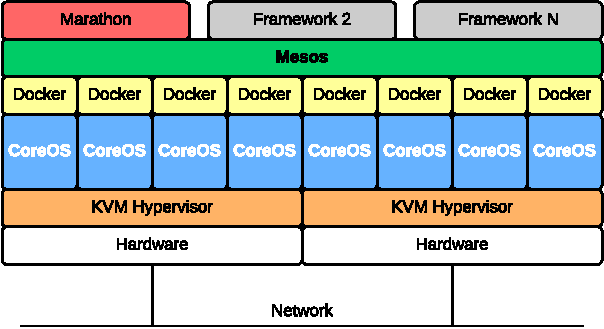
\includegraphics[scale=1]{plataforma}
      \caption{Plataforma de explotación}
\end{figure}

\textbf{¿Cómo?} El grueso del trabajo no se centra en la explotación de la plataforma sino en la automatización de su despliegue. Se detallará el proceso completo, desde el servidor vacío que nos entrega el fabricante hasta la primera ejecución de un trabajo en el \emph{framework} de \emph{Marathon}.\\

Para realizar la automatización se ha creado una plataforma paralela de arranque, o \emph{bootstrapping}, compuesta por cinco elementos funcionales que han sido encapsulados como microservicios dentro de contenedores de \emph{Docker}. El siguiente esquema simplificado conecta con el anterior esquema de la plataforma de explotación:

\begin{figure}[h]
  \centering
    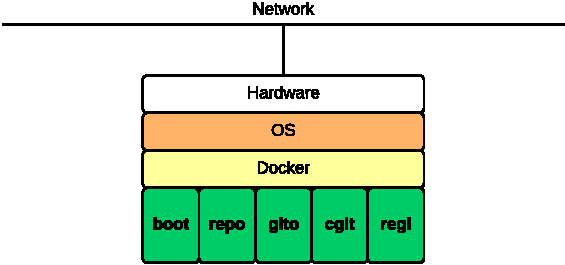
\includegraphics[scale=1]{boot_platform}
      \caption{Plataforma de arranque}
\end{figure}

Más adelante se detallará el rol de cada uno de los cinco contenedores, su proceso de construcción y cómo interactúan entre ellos para aprovisionar los servidores y desplegar los servicios de la plataforma de explotación.

En el contexto de este trabajo entendemos por \emph{'aprovisionamiento de un sistema'} el conjunto de acciones que se deben realizar para disponer de un equipo, ya sea físico o virtual, con un mínimo sistema operativo instanciado y accesible a nivel TCP/IP\@. No se trata de dar mucha inteligencia al sistema de aprovisionamiento, sino de consensuar un modelo sencillo y predecible que resulte eficaz en su funcionamiento y simple de mantener.

Una vez aprovisionados, los sistemas sirven de base sobre la que podemos desplegar servicios. Los servicios determinan el rol o la razón de ser de cada equipo. Si bien en la fase de aprovisionado este rol se perfila sutilmente, no es hasta la fase de despliegue donde se definen con exactitud las funciones de cada equipo y las interrelaciones entre los mismos. Usaremos herramientas como \emph{r10k} y \emph{puppet}.

Empezaremos viendo algunos detalles sobre la plataforma de explotación y seguiremos con el funcionamiento de la plataforma de \emph{bootstrapping}.
\end{intro}

\pagestyle{fancy}

%----------------------------
% Plataforma de explotación:
%----------------------------

\chapter{Plataforma de explotación}
\section{Hardware}
Para el proyecto se han utilizado 2 equipos hipervisores de iguales características. Cada equipo simula un rack que contiene 4 servidores. Algunos de los \emph{frameworks} que pueden ser ejecutados en la plataforma tienen consciencia de rack (\emph{rack awareness}) y distribuyen réplicas de los datos de manera que optimizan el uso de la red (\emph{data locality}) y minimizan el riesgo de pérdida.

Los equipos tienen las siguientes características:

\begin{table}[h]
  \centering
  \begin{tabular}{l|c|c|}
    \hline
    \multicolumn{1}{|c|}{\textbf{Componente}}                       & \textbf{Cantidad} & \textbf{Precio unid.}  \\ \hline
    \multicolumn{1}{|l|}{Placa base Intel DQ77KB Thin Mini-ITX}     & 2                 & 106,23 \euro           \\ \hline
    \multicolumn{1}{|l|}{Procesador Intel Xeon E3-1265Lv2 QuadCore} & 2                 & 344,93 \euro           \\ \hline
    \multicolumn{1}{|l|}{16GB (8GB x2) Crucial DDR3 1600MHz}        & 2                 & 141,30 \euro           \\ \hline
    \multicolumn{1}{|l|}{128GB SSD Crucial mSATA}                   & 2                 & 78,28 \euro            \\ \hline
    \multicolumn{1}{|l|}{Carcasa Thin Mini-ITX Akasa Euler}         & 2                 & 105,80 \euro           \\ \hline
    \multicolumn{1}{|l|}{Cisco SLM2008T-EU 8 x 10/100/1000}         & 1                 & 114,75 \euro           \\ \hline
                                                                    & \textbf{Total}    & \textbf{1667,83 \euro} \\ \cline{2-3}
  \end{tabular}
  \caption{Coste del material}
\end{table}

Cada equipo dispone de dos tarjetas de red. En el siguiente esquema se puede apreciar el conexionado físico y lógico. La ONT es un terminal óptico de red que conecta con la red de fibra del operador Movistar, sobre la VLAN 6 se establece una conexión PPPoE para datos y la VLAN 3 se reserva para voz. Los detalles de conexión con el operador no tienen mayor interés para este trabajo.

\begin{figure}[h]
  \centering
    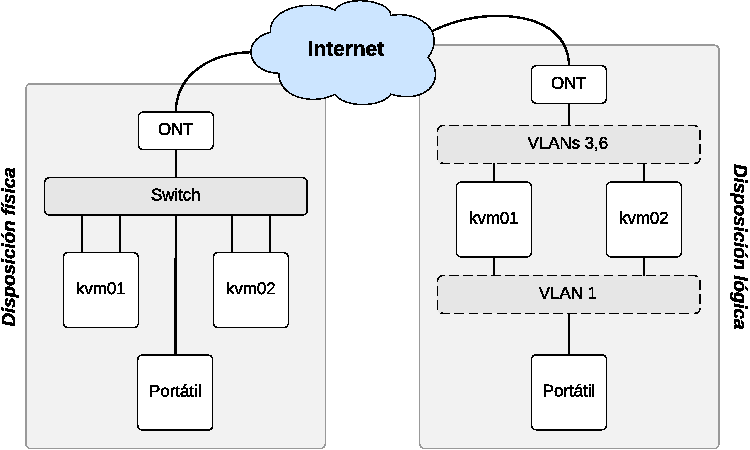
\includegraphics[scale=1]{layout}
      \caption{Disposición de la red}
\end{figure}

El portátil va a ser el equipo que contenga la plataforma de \emph{bootstrapping} que veremos en el segundo capítulo.

\section{Network}

La red se divide en externa e interna. La red externa es la que nos proporciona nuestro operador y normalmente nuestra capacidad para influir sobre su diseño es limitada o nula, por lo que tenemos que adaptarnos a ella. Para realizar este trabajo se ha utilizado una red doméstica FTTH de Movistar.

La red interna es la red sobre la que desplegaremos tanto la plataforma de explotación como la plataforma de \emph{bootstrapping}. Una red interna es suficiente para la simulación de este proyecto, pero en casos con carga real hay que separar las redes en función de su carga y requisitos de seguridad. Por ejemplo, podríamos dedicar una red exclusivamente a tecnologías de almacenamiento de datos.

En la siguiente figura se pueden apreciar los distintos elementos de red que conectan el mundo virtual con el mundo físico.

\begin{figure}[h]
  \centering
    \includegraphics[scale=1]{sdnet}
      \caption{Red definida mediante software}
\end{figure}

La red se define mediante software y a lo largo de distintas fases coordinadas por la plataforma de \emph{bootstrapping}. En el esquema se han coloreado de forma distinta los elementos de red en función de la pieza de software que los configura.

\section{Software}

La pila o \emph{stack} de software es aparentemente compleja, sin embargo, se repite para cada nodo del cluster de manera que el escalado se convierte en una tarea sencilla. En la siguiente figura se pueden apreciar con algo más de detalle los distintos componentes que constituyen la plataforma de explotación.

\begin{figure}[h]
  \centering
    \includegraphics[scale=0.75]{detailed_stack}
      \caption{Pila de software}
\end{figure}

Para conseguir alta disponiblilidad (HA) en un cluster real serían necesarias 3 o 5 instancias de \emph{Mesos Master} y 3 o 5 instancias de \emph{Zookeeper}. En este caso, para la prueba de concepto en esta maqueta es suficiente con una única instancia de cada uno. \emph{Zookeeper} y \emph{Etcd} son componentes que ofrecen funcionalidades muy similares y a la larga \emph{Zookeeper} será reemplazado.

A continuación, veremos algunos detalles sobre cada uno de los componentes más importantes.

\subsection{KVM}

KVM (Kernel-based Virtual Machine) es una respuesta a la necesidad de implementar virtualización completa con Linux. Se compone de un módulo del núcleo (\emph{kvm.ko}) y herramientas en el espacio de usuario. El componente KVM para el núcleo está incluido en Linux desde la versión 2.6.20.

KVM permite ejecutar máquinas virtuales utilizando imágenes de disco que contienen sistemas operativos. Cada máquina virtual tiene su propio hardware virtualizado: tarjetas de red, discos duros, CPUs, etc.

Una de las características que KVM posee es la estrategia de \emph{overcommit}. En este proyecto ésta se aplica en dos recursos: CPU y memoria. En ambos casos consiste en comprometerse a abastecer con más recursos de los que físicamente dispone el host.

\subsection{CoreUp}

\emph{CoreUp} es un script de 300 líneas escrito en \emph{Bash}. Su cometido principal es preparar el entorno para instanciar \emph{CoreOS}, es la `argamasa' entre KVM y \emph{CoreOS}. Una vez ejecutado no queda residente en memoria. Se encarga de:

\begin{itemize}
  \item Verificar que el entorno es el adecuado para instanciar los servidores virtuales.
  \item Descargar la imagen de disco de CoreOS. Esta imagen se sirve desde el contenedor \emph{data01} para evitar la dependencia con internet.
  \item Incrementar el tamaño de disco de la imagen descargada a 20GB ya que el tamaño por defecto es únicamente de 3GB.
  \item Generar de forma dinámica la configuración de \emph{cloud-config} para las distintas instancias de CoreOS.
  \item Generar dispositivos TAP de red (capa 2) para interconectar las VMs con el host anfitrión.
  \item Generar direcciones MAC deterministas (siempre las mismas) para evitar colisiones entre las máquinas virtuales.
  \item Instanciar 4 servidores virtuales en cada hipervisor.
\end{itemize}

A continuación vemos como \emph{CoreUp} inicia por primera vez la máquina virtual \emph{core01}.
\\

\begin{lstlisting}[style=dnsmasq]
[root@kvm01 ~]# coreup core01
Checking VM is not running...                                                           [  OK  ]
Checking hostname is not in use...                                                      [  OK  ]
Checking VM limit is not reached...                                                     [  OK  ]
Downloading CoreOS image file...                                                        [  OK  ]
Resizing CoreOS disk image...                                                           [  OK  ]
Generating cloud-config...                                                              [  OK  ]
Generating TAP interfaces...                                                            [  OK  ]
Starting the virtual machine...                                                         [  OK  ]
Testing SSH port...                                                                     [  OK  ]
Restarting after first boot...                                                          [  OK  ]
Checking VM is not running...                                                           [  OK  ]
Checking hostname is not in use...                                                      [  OK  ]
Checking VM limit is not reached...                                                     [  OK  ]
Generating cloud-config...                                                              [  OK  ]
Generating TAP interfaces...                                                            [  OK  ]
Starting the virtual machine...                                                         [  OK  ]
Testing SSH port...                                                                     [  OK  ]
\end{lstlisting}

\subsection{CoreOS}

\emph{CoreOS} es una distribución de Linux minimalista. Los servicios que proporciona están orientados a cimentar infraestructuras de clusters. La distribución promueve el uso de contenedores como modelo de distribución de software abandonando así los tradicionales gestores de paquetes. Los servicios de \emph{CoreOS} que usaremos para este proyecto son \emph{Etcd}, \emph{Fleet} y \emph{Docker}.

\subsubsection{Etcd}

\emph{Etcd} es una base de datos de clave valor que utiliza el algoritmo de consenso \emph{Raft} para realizar la elección automática de su master. Los datos almacenados en \emph{Etcd} se distribuyen y replican de forma automática, de manera que los cambios se reflejan en todo el cluster.

Por sus características, se utiliza en el campo de la localización de servicios y configuraciones compartidas. Sus bajos tiempos de convergencia (todos los servidores acuerdan el valor de las claves) la hacen ideal en entornos donde se requiere tolerancia a fallos.

En la maqueta podemos consultar cuál de los nodos ha sido elegido líder del cluster ejecutando el siguiente comando:\\

\begin{lstlisting}[style=dnsmasq]
core@core01# curl -L http://127.0.0.1:4001/v2/leader
http://core03:7001
\end{lstlisting}

También podemos consultar la lista de nodos que son miembros del cluster de \emph{Etcd} ejecutando el siguiente comando:\\

\begin{lstlisting}[style=dnsmasq]
core@core01# curl -sL http://127.0.0.1:4001/v2/machines | sed s/,\ /\\n/g
http://core03:4001
http://core04:4001
http://core05:4001
http://core06:4001
http://core07:4001
http://core08:4001
http://core01:4001
http://core02:4001
\end{lstlisting}

\subsubsection{Fleet}

\emph{Fleet} es una herramienta de gestión de clusters que utiliza \emph{Etcd} para la compartición de configuraciones. \emph{Fleet} controla los sistemas de inicialización de servicios (\emph{systemd}) de todos los nodos del cluster, proporcionando así una gestión unificada.

Podemos consultar el listado de nodos que forman parte del cluster de \emph{Fleet} con el siguiente comando:\\

\begin{lstlisting}[style=dnsmasq]
core@core01# fleetctl list-machines
MACHINE   IP    METADATA
2382b63a... 192.168.1.140 host=core06
2d5dc467... 192.168.1.62  host=core08
35b394af... 192.168.1.98  host=core05
35e7ee19... 192.168.1.119 host=core04
747ce9e7... 192.168.1.89  host=core03
99a44c29... 192.168.1.143 host=core01
a6668efd... 192.168.1.54  host=core02
f469c6df... 192.168.1.141 host=core07
\end{lstlisting}

También podemos consultar el estado de los servicios controlados por \emph{Fleet} utilizando el siguiente comando:\\

\begin{lstlisting}[style=dnsmasq]
core@core01# fleetctl list-units
UNIT      MACHINE       ACTIVE  SUB
marathon.service     99a44c29.../192.168.1.143 active  running
mesos-master.service 99a44c29.../192.168.1.143 active  running
mesos-slave.service  2382b63a.../192.168.1.140 active  running
mesos-slave.service  2d5dc467.../192.168.1.62  active  running
mesos-slave.service  35b394af.../192.168.1.98  active  running
mesos-slave.service  35e7ee19.../192.168.1.119 active  running
mesos-slave.service  747ce9e7.../192.168.1.89  active  running
mesos-slave.service  99a44c29.../192.168.1.143 active  running
mesos-slave.service  a6668efd.../192.168.1.54  active  running
mesos-slave.service  f469c6df.../192.168.1.141 active  running
zookeeper.service    a6668efd.../192.168.1.54  active  running
\end{lstlisting}

En la plataforma de explotación se utiliza \emph{Fleet} para arrancar todos los servicios relacionados con \emph{Mesos} incluidos sus \emph{frameworks}, por lo tanto también \emph{Marathon}.

\subsubsection{Docker}

\emph{Docker} es un proyecto de código abierto que automatiza el despliegue de aplicaciones encapsulándolas dentro de contenedores de software. \emph{Docker} utiliza tecnologías de aislamiento de recursos, como los \emph{cgroups} o los \emph{namespaces}, que se encuentran disponibles en el kernel de Linux.

En una misma instancia de Linux se pueden crear múltiples contenedores, independientes los unos de los otros y sin la sobrecarga que supondría crear máquinas virtuales.

La visión del sistema operativo que tiene la aplicación queda completamente aislada, incluyendo el árbol de procesos, la pila de red, los sistemas de ficheros y los identificadores de usuarios, así como los recursos de CPU, memoria, I/O y red.

Las principales ventajas que aporta la containerización son:
\begin{itemize}
  \item \textbf{Inmutabilidad:} Entornos estáticos para albergar las aplicaciones y proporcionar fiabilidad en el despliegue de las mismas cuando éste se realiza en plataformas distintas a la de desarollo.
  \item \textbf{Portabilidad:} Los contenedores son artefactos ejecutables que se pueden mover, almacenar, copiar o destruir con facilidad.
  \item \textbf{Desacoplamiento:} Las aplicaciones más complejas se componen a base de múltiples aplicaciones ligeras que se interrelacionan entre sí (microservicios).
\end{itemize}

En cualquier instancia de \emph{CoreOS} de la maqueta se puede consultar el listado de imágenes de contenedores descargadas y listas para ser instanciadas:\\

\begin{lstlisting}[style=dnsmasq]
core@core01# docker images
REPOSITORY                          TAG          IMAGE ID           CREATED           VIRTUAL SIZE
regi01.demo.lan:5000/marathon       latest       beccb9c8de89       5 weeks ago       1.248 GB
regi01.demo.lan:5000/marathon       v0.7.5       beccb9c8de89       5 weeks ago       1.248 GB
regi01.demo.lan:5000/mesos-slave    0.20.1       cb1584229bc1       4 months ago      1.168 GB
regi01.demo.lan:5000/mesos-slave    latest       cb1584229bc1       4 months ago      1.168 GB
regi01.demo.lan:5000/mesos-master   0.20.1       fd7f7e5c4513       4 months ago      1.168 GB
regi01.demo.lan:5000/mesos-master   latest       fd7f7e5c4513       4 months ago      1.168 GB
\end{lstlisting}

También podemos consultar el listado de contenedores instanciados:\\

\begin{lstlisting}[style=dnsmasq]
core@core01# docker ps
CONTAINER ID  IMAGE                COMMAND              CREATED        STATUS       NAMES
b709ae465b18  mesos-master:0.20.1  mesos-master --ip=1  10 hours ago   Up 10 hours  mesos_master
f1cfa94270cb  marathon:latest      ./bin/start --maste  10 hours ago   Up 10 hours  marathon
e18163eab926  mesos-slave:0.20.1   mesos-slave --ip=19  10 hours ago   Up 10 hours  mesos_slave
\end{lstlisting}

\subsection{Mesos}

\emph{Mesos} proporciona una capa de abstracción sobre los recursos de CPU, de memoria y de disco presentes en flotas de servidores. Esta capa ligera sirve de base sobre la que construir sistemas distribuidos, elásticos y tolerantes a fallos.

De forma análoga a la relación que se establece entre las aplicaciones, el kernel y los recursos de hardware, \emph{Mesos} sirve de gestor de recursos y planificador de tareas entre los \emph{frameworks} y los recursos hardware del centro de datos. En otras palabras, \emph{Mesos} es el kernel del centro de datos.

\emph{Mesos} ofrece recursos a los \emph{frameworks} y éstos pueden aceptar o declinar las ofertas. En caso de ser aceptadas, es tarea de los \emph{frameworks} planificar los trabajos que se van a llevar a cabo con los recursos adquiridos. Las ofertas son bloqueantes lo que significa que no se ofrecerán los mismos recursos a dos \emph{frameworks} distintos simultáneamente. Por todo ello, también se describe a \emph{Mesos} como un `planificador pesimista de dos niveles'.

En la maqueta del proyecto podemos consultar el listado de tareas en ejecución utilizando un contenedor creado específicamente para ejecutar comandos en \emph{Mesos}:\\

\begin{lstlisting}[style=dnsmasq]
# docker run -it --rm --env MESOS_MASTER=zk://core02:2181/mesos h0tbird/mcli mesos ps

   TIME   STATE   RSS    CPU  %MEM          COMMAND          USER                        ID
 0:00:00    R    0.00 B   0   0.00  sh -c 'nc -p $PORT0...'  root  hostname.11e4-8c27-0242ac110002
 0:00:00    R    0.00 B   0   0.00  sh -c 'nc -p $PORT0...'  root  hostname.11e4-8c27-0242ac110002
 0:00:00    R    0.00 B   0   0.00  sh -c 'nc -p $PORT0...'  root  hostname.11e4-8c27-0242ac110002
 0:00:00    R    0.00 B   0   0.00  sh -c 'nc -p $PORT0...'  root  hostname.11e4-8c27-0242ac110002
 0:00:00    R    0.00 B   0   0.00  sh -c 'nc -p $PORT0...'  root  hostname.11e4-8c27-0242ac110002
 0:00:00    R    0.00 B   0   0.00  sh -c 'nc -p $PORT0...'  root  hostname.11e4-8c27-0242ac110002
 0:00:00    R    0.00 B   0   0.00  sh -c 'nc -p $PORT0...'  root  hostname.11e4-8c27-0242ac110002
 0:00:00    R    0.00 B   0   0.00  sh -c 'nc -p $PORT0...'  root  hostname.11e4-8c27-0242ac110002
\end{lstlisting}

\subsubsection{Marathon}

\emph{Marathon} es un \emph{framework} de \emph{Mesos} especialmente diseñado para ejecutar aplicaciones que tienen una esperanza de vida larga, como por ejemplo, un servidor web \emph{Apache} o una base de datos de clave valor \emph{Redis}.

\emph{Marathon} y \emph{Fleet} son herramientas similares. Las dos son consideradas \emph{`init systems'} distribuidos; sin embargo, \emph{Marathon} ofrece más prestaciones que \emph{Fleet}. Es por ello que el papel de \emph{Fleet} queda relegado a arrancar los servicios de \emph{Mesos} y \emph{Marathon}.

\emph{Marathon} proporciona una API REST para arrancar, parar y escalar applicaciones, está escrito en \emph{Scala} y puede funcionar en alta disponibilidad arrancando múltiples instancias.

El siguiente ejemplo muestra cómo arrancar una aplicación muy simple en \emph{Marathon}.\\

\begin{lstlisting}[style=dnsmasq]
curl -s -H "Content-Type: application/json" http://core01:8080/v2/apps -d \
  ' {
      "id": "hostname",
      "cmd": "nc -p $PORT0 -ll -e hostname",
      "cpus": 0.2,
      "mem": 2.0,
      "instances": 1,
      "container": {
        "type": "DOCKER",
        "docker": {
          "image": "busybox:latest"
        }
      }
    }
  ' | jq '.'
\end{lstlisting}

%-------------------------
% Plataforma de arranque:
%-------------------------

\chapter{Plataforma de arranque}

%----------------
% Bootstrapping:
%----------------

\chapter{Secuencia de arranque}

\section{Pre arranque}
Al pulsar el botón de encendido en un servidor, se inicia el proceso de pre arranque o \emph{`pre boot sequence'}. En el mismo instante en que existe diferencia de potencial, se empiezan a ejecutar una serie de procedimientos basados en hardware que realizan comprobaciones funcionales de la propia electrónica del equipo.

Aquellos componentes electrónicos que dispongan de capacidades \emph{POST} (\emph{Power-On Self Test}), ejecutarán sus rutinas como parte de la secuencia de pre arranque. Si se produjera un error en esta fase, se cancelaría la siguiente fase de arranque y se notificaría el hecho mediante señales acústicas, leds o displays, si el equipo dispone de ellos.

\begin{figure}[h]
  \centering
    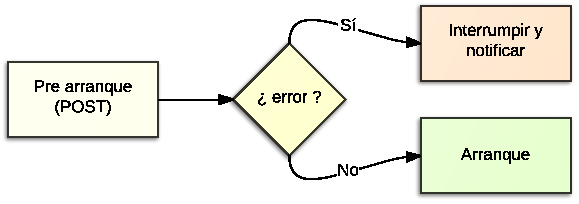
\includegraphics[scale=1]{pre_arranque}
      \caption{Pre arranque}
\end{figure}

\section{Arranque}
Durante el arranque o \emph{`bootstrapping'} se pasa por una serie de fases encadenadas. Cada fase se encarga de preparar el entorno para cargar y ejecutar la siguiente de manera que, en cada fase, se aumentan las funcionalidades y la complejidad del código ejecutado.

La lógica y los datos de las funcionalidades más básicas constituyen el \emph{firmware} del equipo. Éste se encuentra a salvo en direcciones fijas dentro de chips de memoria persistente (\emph{ROM}, \emph{EPROM}, \emph{Flash}) y suele limitarse a proporcionar servicios a una capa superior de software. La vieja y conocida \emph{BIOS} (\emph{Basic Input/Output System}) o la nueva \emph{UEFI} (\emph{Unified Extensible Firmware Interface}), son buenos ejemplos de ello.

Una de las funcionalidades del \emph{firmware} que más nos interesa es la de \emph{`first-stage boot loader'} que se ocupa de localizar, recuperar, cargar en memoria y transferir el control de ejecución al software de arranque o \emph{`bootstrap program'}.

Ejemplos típicos de aplicaciones que encontramos en la categoría de software de arranque son: \emph{LILO}, \emph{GRUB}, \emph{Syslinux}, \emph{PXELinux.0} e incluso podríamos considerar al mismo \emph{kernel} de Linux en esta categoría. Los cuatro primeros se utilizan como \emph{`second-stage boot loaders'} y permiten al usuario gestionar una gran diversidad de opciones de arranque.

\begin{figure}[h]
  \centering
    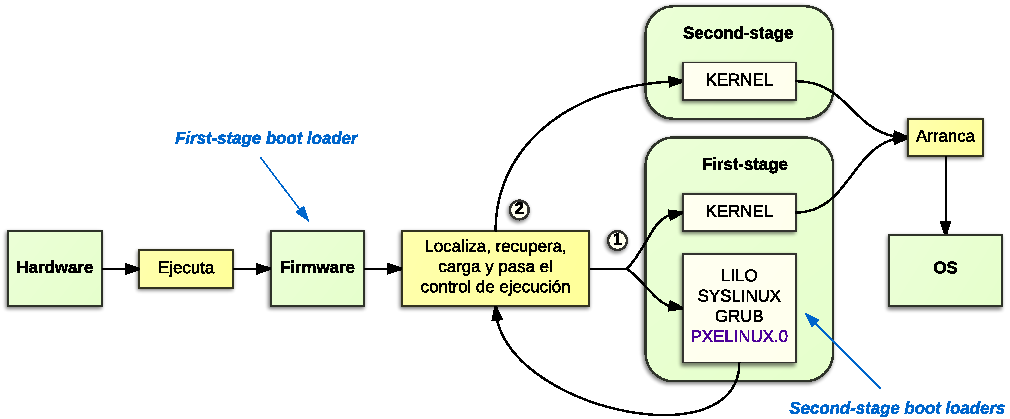
\includegraphics[scale=0.9]{arranque}
      \caption{Arranque}
\end{figure}

\emph{LILO}, \emph{GRUB} y \emph{Syslinux} suelen encontrarse ubicados en el \emph{MBR} (\emph{Master Boot Record}) del dispositivo de arranque, pudiendo ser éste un disco duro, un disquete o un \emph{DVD}. \emph{PXELinux.0} es una variante de \emph{Syslinux} que, a diferencia de los anteriores, se encuentra ubicado en un equipo remoto de la red local.

Puesto que no es lo mismo recuperar el software de arranque desde un \emph{MBR} que desde un equipo remoto, el \emph{firmware} que quiera ejecutar \emph{PXELinux.0}, va a tener que implementar una solución específica. A continuación veremos las tecnologías que lo hacen posible.

\subsection{PXE}
\emph{PXE} (\emph{Pre-Execution Environment}) extiende las funcionalidades del \emph{firmware} dotándolo de capacidades comunicativas gracias a la inclusión de los protocolos \emph{IPv4}, \emph{UDP}, \emph{DHCP} y \emph{TFTP}, estos dos últimos con leves modificaciones. Con estas extensiones, el \emph{firmware} es capaz de localizar, descargar y transferir el control de ejecución al software de arranque \emph{PXELinux.0}, también conocido con el nombre genérico de \emph{NBP} (\emph{Network Bootstrap Program}), que se encuentra ubicado en otro equipo de la red local.

De forma resumida, la mecánica del protocolo \emph{PXE} funciona de la siguiente manera. El cliente inicia el protocolo mediante un broadcast conocido como \emph{DHCPDISCOVER} que contiene unas extensiones (opciones 128 a 135 del \emph{RFC} 4578) que identifican la solicitud como procedente de un equipo que implementa el protocolo \emph{PXE}. En el log del servidor que recibe la solicitud podemos ver los siguientes detalles:\\

\begin{lstlisting}[style=dnsmasq]
DHCPDISCOVER(eth1) 00:30:1b:a0:6f:cc
requested options: 1:netmask, 2:time-offset, 3:router, 5, 6:dns-server,
requested options: 11, 12:hostname, 13:boot-file-size, 15:domain-name,
requested options: 16:swap-server, 17:root-path, 18:extension-path,
requested options: 43:vendor-encap, 54:server-identifier, 60:vendor-class,
requested options: 67:bootfile-name, (*@\textcolor{softred}{128}@*), (*@\textcolor{softred}{129}@*), (*@\textcolor{softred}{130}@*), (*@\textcolor{softred}{131}@*), (*@\textcolor{softred}{132}@*),
requested options: (*@\textcolor{softred}{133}@*), (*@\textcolor{softred}{134}@*), (*@\textcolor{softred}{135}@*)
\end{lstlisting}

Asumiendo que en la red existe un servidor \emph{DHCP} o un proxy \emph{DHCP} que también implementa las mismas extensiones del protocolo \emph{DHCP}, el servidor envía al cliente una lista de servidores de arranque (el servidor redirige al cliente) y el nombre del fichero de arranque que el cliente tiene que descargar (\emph{pxelinux.0} en nuestro caso).\\

\begin{lstlisting}[style=dnsmasq]
dnsmasq-dhcp[15]: DHCPOFFER(eth1) 192.168.1.51 00:30:1b:a0:6f:cc
dnsmasq-dhcp[15]: (*@\textcolor{softred}{next server: 192.168.1.2}@*)
dnsmasq-dhcp[15]: sent size:  1 option: 53 message-type  2
dnsmasq-dhcp[15]: option: 54 server-identifier  192.168.1.2
dnsmasq-dhcp[15]: option: 51 lease-time  12h
dnsmasq-dhcp[15]: option: 58 T1  6h
dnsmasq-dhcp[15]: option: 59 T2  10h30m
dnsmasq-dhcp[15]: option: 67 (*@\textcolor{softred}{bootfile-name  pxelinux.0}@*)
dnsmasq-dhcp[15]: option:  1 netmask  255.255.255.0
dnsmasq-dhcp[15]: option: 28 broadcast  192.168.1.255
dnsmasq-dhcp[15]: option:  3 router  192.168.1.1
dnsmasq-dhcp[15]: option:  6 dns-server  192.168.1.2
dnsmasq-dhcp[15]: available DHCP range: 192.168.1.50 -- 192.168.1.150
\end{lstlisting}

A continuación, el cliente utiliza \emph{TFTP} para descargar el \emph{NBP} de uno de los servidores de arranque. Finalmente, el \emph{firmware} del cliente transfiere el control de ejecución a la imagen descargada.\\

\begin{lstlisting}[style=dnsmasq]
dnsmasq-tftp[15]: (*@\textcolor{softred}{sent /tftpboot/pxelinux.0 to 192.168.1.51}@*)
\end{lstlisting}

\subsubsection{PXELinux.0}
\emph{PXELinux.0} actua como \emph{`Second Stage Boot Loader'} permitiendo localizar, descargar y pasar el control de ejecución al \emph{kernel} de Linux y a su correspondiente \emph{initramfs} (\emph{Initial RAM File System}). \emph{PXELinux.0} comunica al \emph{kernel} la dirección de memoria en la que ha cargado el \emph{initramfs}. La ejecución del \emph{kernel} puede ser parametrizada mediante un fichero de configuración que además, permite definir menús interactivos. El primer fichero que \emph{PXELinux.0} intenta descargar del servidor \emph{TFTP} es por tanto, su propio fichero de configuración.

Cada cliente puede disponer de su propio fichero de configuración. El nombre del fichero de cada equipo queda determinado por su dirección \emph{MAC} o la conversión a hexadecimal de su dirección \emph{IP}. Si no existe fichero alguno con ese nombre, se procede a eliminar un dígito hexadecimal del final del nombre y se repite la búsqueda sucesivamente tal y como se muestra en la siguiente captura:\\

\begin{lstlisting}[style=dnsmasq]
dnsmasq-tftp[15]: file /tftpboot/pxelinux.cfg/01-00-30-1b-a0-6f-cc not found
dnsmasq-tftp[15]: file /tftpboot/pxelinux.cfg/C0A80233 not found
dnsmasq-tftp[15]: file /tftpboot/pxelinux.cfg/C0A8023 not found
dnsmasq-tftp[15]: file /tftpboot/pxelinux.cfg/C0A802 not found
dnsmasq-tftp[15]: file /tftpboot/pxelinux.cfg/C0A80 not found
dnsmasq-tftp[15]: file /tftpboot/pxelinux.cfg/C0A8 not found
dnsmasq-tftp[15]: file /tftpboot/pxelinux.cfg/C0A not found
dnsmasq-tftp[15]: file /tftpboot/pxelinux.cfg/C0 not found
dnsmasq-tftp[15]: file /tftpboot/pxelinux.cfg/C not found
dnsmasq-tftp[15]: (*@\textcolor{softred}{sent /tftpboot/pxelinux.cfg/default to 192.168.1.51}@*)
dnsmasq-tftp[15]: (*@\textcolor{softred}{sent /tftpboot/menu.c32 to 192.168.1.51}@*)
\end{lstlisting}

Si finalmente no se encuentra ninguna configuración, se utilizará el fichero por defecto llamado \emph{`default'}. Para la realización de este proyecto se ha definido que todos los equipos físicos dispongan de configuración específica y que las máquinas virtuales usen la configuración por defecto. Por ejemplo, al equipo físico que realizará funciones de hipervisor se le aplica la siguiente configuración:\\

\begin{lstlisting}[style=dnsmasq]
DEFAULT menu.c32
PROMPT 0
TIMEOUT 100
ONTIMEOUT local

MENU TITLE Main Menu

LABEL local
  MENU LABEL Boot local hard drive
  LOCALBOOT 0

LABEL install
  MENU LABEL Unattended CentOS 7 installation
  KERNEL images/centos/7/x86_64/vmlinuz
  IPAPPEND 2
  APPEND initrd=images/centos/7/x86_64/initrd.img rd.driver.pre=loop
         inst.repo=http://data01.demo.lan/centos/7/os/x86_64/
         inst.ks=http://data01.demo.lan:/kickstarts/akasa.ks
         inst.geoloc=0 inst.text
\end{lstlisting}

Tras descargar el fichero de configuración de \emph{PXELinux.0} se procede a su interpretación. La primera línea (\emph{DEFAULT menu.c32}) provoca la descarga mediante \emph{TFTP} de otro binario cuya única función es presentar un menú interactivo en la consola del sistema. El resto del fichero contiene la configuración de dicho menú. Cada elemento seleccionable contiene la información necesaria para localizar a una pareja de \emph{kernel} y \emph{initramfs} así como los parámetros adicionales que se le quieran entregar al \emph{kernel} en el momento de su ejecución.

El aspecto del menú que nos presenta \emph{menu.c32} es el siguiente:\\

\begin{lstlisting}[style=dnsmasq]
                   +----------------------------------------------------------+
                   |                        Main Menu                         |
                   +----------------------------------------------------------+
                   | Boot local hard drive                                    |
                   | Unattended CentOS 7 installation                         |
                   |                                                          |
                   |                                                          |
                   |                                                          |
                   |                                                          |
                   |                                                          |
                   |                                                          |
                   |                                                          |
                   |                                                          |
                   |                                                          |
                   |                                                          |
                   +----------------------------------------------------------+

                                     Press [Tab] to edit options

                                    Automatic boot in 7 seconds...
\end{lstlisting}

Si pulsamos \emph{[Tab]} sobre la opción \emph{`Unattended CentOS 7 installation'} podremos editar la línea del comando que se ejecuta al seleccionar esta opción:\\

\begin{lstlisting}[style=dnsmasq]
> images/centos/7/x86_64/vmlinuz initrd=images/centos/7/x86_64/initrd.img rd.driver.pre=loop inst.
repo=http://data01.demo.lan/centos/7/os/x86_64/ inst.ks=http://data01.demo.lan:/kickstarts/akasa.ks
inst.geoloc=0 inst.text BOOTIF=01-00-30-1b-a0-6f-cc
\end{lstlisting}

Los parámetros que no tienen el prefijo \emph{`inst'} serán interpretados directamente por el \emph{kernel} o por el subsistema \emph{Dracut}. Los parámetros que si que tienen el prefijo \emph{`inst'} van a ser interpretados más adelante por el instalador \emph{Anaconda}. El parámetro \emph{BOOTIF} que aparece al final, es consecuencia de la opción \emph{IPAPPEND 2} que hemos añadido en la configuración de \emph{PXELinux.0}. La dirección \emph{MAC} que aparece, corresponde con la interfície de red que ha iniciado el proceso \emph{PXE}, este valor también será usado más adelante por \emph{Anaconda}.

En el siguiente esquema se representan las interacciones que se establecen entre los gestores de arranque del servidor que queremos aprovisionar \emph{kvm01} y el contenedor de arranque \emph{boot01}:\\

\begin{figure}[h]
  \centering
    \includegraphics[scale=0.85]{bootstrap_1}
      \caption{Gestor de arranque}
\end{figure}

\subsection{Dracut}
Con el \emph{kernel} y el \emph{initramfs} ya cargados en memoria, \emph{PXELinux.0} entrega el control de ejecución, la dirección de memoria donde se encuentra el \emph{initramfs} y los parámetros de arranque al \emph{kernel} de Linux. El \emph{kernel} se descomprime a sí mismo y extrae el \emph{initramfs} (que se encuentra en formato \emph{cpio}) montándolo en el sistema de archivos raíz o \emph{`root file system (rootfs)'} para, finalmente, transferir el control de ejecución al binario \emph{/init} que ahora se encuentra en la raíz del nuevo \emph{rootfs}.

En este contexto \emph{Dracut} tiene dos roles. Por un lado, es la herramienta de línea de comandos que se usa para crear el \emph{initramfs} y por otro lado, es el propio subsistema que se encierra dentro del \emph{initramfs} y que es invocado al ejecutar \emph{/init}. La única tarea del subsistema \emph{Dracut} es localizar, cargar y conmutar a la imagen final de \emph{rootfs} que contiene el instalador \emph{Anaconda} y que se usará durante el posterior proceso de instalación.

\subsubsection{Herramienta de línea de comandos}
Normalmente no es necesario crear un \emph{initramfs} a medida. Sin embargo, uno de los servidores que se han utilizado para realizar pruebas, necesita soporte específico para una tarjeta de red \emph{Nvidia}.
Para generar el nuevo \emph{initramfs} que incorpora el driver obsoleto \emph{forcedeth}, se ha utilizado un contenedor de \emph{Docker} tal y como se muestra a continuación:\\

\begin{lstlisting}[style=dnsmasq]
$ docker run -it --rm -e KVER='3.10.0-123' -v ${PWD}/initramfs:/initramfs h0tbird/centos bash -c "
sed -i '/exclude/d' /etc/yum.conf && \
yum clean all && \
yum -y update && \
yum install -y kernel-\${KVER}.el7 *dracut* vi tar gzip dd rpcbind nfs-utils \
http://elrepo.org/linux/elrepo/el7/x86_64/RPMS/kmod-forcedeth-0.64-1.el7.elrepo.x86_64.rpm && \
depmod \${KVER}.el7.x86_64 && \
echo loop > /usr/lib/modules-load.d/loop.conf && \
echo 'options loop max_loop=8' > /usr/lib/modprobe.d/eightloop.conf && \
dracut -v -m 'anaconda base plymouth kernel-modules' --add-drivers forcedeth \
-f /initramfs/forcedeth.img --kver \${KVER}.el7.x86_64"
\end{lstlisting}

Tras ejecutar el comando anterior, aparecerá un nuevo subdirectorio en el directorio actual con el nombre \emph{initramfs}. Dentro se encuentra el \emph{initramfs} que acabamos de generar. Para listar su contenido podemos ejecutar \emph{`lsinitcpio initramfs/forcedeth.img'}.

\subsubsection{Subsistema Dracut}
Muchas distribuciones de Linux utilizan un único \emph{kernel} genérico con el que pretenden arrancar la más amplia variedad de hardware posible.
Los controladores de dispositivos para esta imagen genérica se incluyen como módulos de carga dinámica o \emph{`loadable modules'} ya que no es posible compilarlos todos de forma estática en el \emph{kernel} sin hacerlo demasiado grande como para arrancarlo desde sistemas con poca memoria.

Se plantea entonces el problema de detectar los dispositivos y cargar los módulos necesarios para montar el sistema de ficheros raíz durante el arranque o, para el caso, determinar dónde se encuentra y qué constituye el \emph{rootfs}.

La misión principal del subsitema \emph{Dracut} es montar el \emph{rootfs} detectando dispositivos y cargando los drivers que sean necesarios para ello.

En el siguiente esquema se representan las interacciones que se establecen entre \emph{Dracut} y el contenedor de datos \emph{data01}:\\

\begin{figure}[h]
  \centering
    \includegraphics[scale=0.85]{bootstrap_2}
      \caption{Dracut}
\end{figure}

\section{Instalación}

\subsection{Anaconda}

\emph{Anaconda} es el programa de instalación usado por \emph{RedHat}, \emph{Fedora} y otras distribuciones de \emph{Linux}. Durante la instalación se detecta y configura el hardware del equipo y se prepara el sistema de ficheros adecuado para cada arquitectura. El instalador permite al usuario instalar y/o actualizar software en el equipo final. Una vez terminada la instalación, es necesario reiniciar el equipor para arrancar el nuevo sistema.

\emph{Anaconda} es un instalador muy completo. Permite instalar desde fuentes locales y remotas como CDs y DVDs o imágenes almacenadas en disco, \emph{NFS}, \emph{HTTP} o \emph{FTP}. Pero la característica más destacable de \emph{Anaconda} para este proyecto es su capacidad para automatizar las instalaciones mediante ficheros \emph{kickstart}.

\subsubsection{Kickstart}

La idea que hay detrás de los ficheros \emph{kickstart} es muy sencilla. Se trata de proporcionar al instalador \emph{Anaconda} un fichero con todas las respuestas a las preguntas que normalmente se hacen durante el proceso de instalación. El objetivo es que la instalación sea totalment desatendida.

Un fichero \emph{kickstart} no es más que un fichero de texto que contiene distintos elementos agrupados por secciones ordenadas. A continuación se muestra un fragmento del fichero \emph{kvm-akasa.ks} utilizado para aprovisionar los hipervisores de este proyecto:\\

\begin{lstlisting}[style=dnsmasq]
install
url --url="http://data01.demo.lan/centos/7/os/x86_64/"
text
keyboard es
lang en_US.UTF-8
eula --agreed
network --bootproto=dhcp --device=bootif --onboot=on
rootpw password
timezone Europe/Madrid --isUtc
services --disabled auditd,avahi-daemon,NetworkManager,postfix,microcode,tuned
services --enabled network,sshd
selinux --disabled
firewall --disabled
repo --name="CentOS" --baseurl=http://data01.demo.lan/centos/7/os/x86_64/
repo --name="Updates" --baseurl=http://data01.demo.lan/centos/7/updates/
repo --name="EPEL" --baseurl=http://data01.demo.lan/centos/7/epel/
repo --name="Misc" --baseurl=http://data01.demo.lan/centos/7/misc/
repo --name="Puppet-products" --baseurl=http://data01.demo.lan/puppet/puppetlabs-products/
repo --name="Puppet-deps" --baseurl=http://data01.demo.lan/puppet/puppetlabs-deps/
ignoredisk --only-use=sda
bootloader --location=mbr
zerombr
clearpart --all --initlabel
part swap --asprimary --fstype="swap" --size=1024
part /boot --fstype xfs --size=200
part / --fstype ext4 --size=1024 --grow
reboot
\end{lstlisting}

En la sección \emph{post} del fichero se le indica a \emph{Anaconda} que utilice \emph{R10K} para instalar el código que posteriormente será utilizado por \emph{Puppet}:\\

\begin{lstlisting}[style=dnsmasq]
% post --log=/root/ks-post-chroot.log
cat << EOF > /etc/r10k.yaml
cachedir: /var/cache/r10k
sources:
 puppet:
  remote: 'http://gito01.demo.lan/cgit/r10k-kvm'
   basedir: /etc/puppet/environments
EOF

rm -rf /etc/puppet
git clone http://gito01.demo.lan/cgit/puppet-config /etc/puppet
rm -rf /etc/puppet/environments/*
/usr/local/bin/r10k deploy environment
\end{lstlisting}

En el siguiente esquema se representan las interacciones que se establecen entre \emph{Anaconda}, el contenedor de datos \emph{data01} y el contenedor de repositorios de código \emph{gito01}:

\begin{figure}[h]
  \centering
    \includegraphics[scale=0.85]{bootstrap_3}
      \caption{Anaconda}
\end{figure}

\subsection{R10K}

\subsection{Puppet}

\emph{R10K} descarga los módulos de \emph{Puppet} y \emph{Puppet} los aplica en el servidor para convertirlo en un hipervisor e instanciar las cuatro máqinas virtuales con \emph{CoreOS}. Dentro de \emph{CoreOS} \emph{Fleet} y \emph{Marathon} se conectan al registro de \emph{Docker} para descargar las imágenes de los contenedores:

\begin{figure}[h]
  \centering
    \includegraphics[scale=0.85]{bootstrap_4}
      \caption{R10K, Puppet y CoreOS}
\end{figure}

%------------------------
% Guía de inicio rápido:
%------------------------

\chapter{Guía de inicio rápido}

%------------
% Biografía:
%------------

\begin{thebibliography}{2}

%% Llibres:  Autor/s (cognoms i inicials dels noms), títol del llibre (en cursiva), editor, ciutat i any de publicació. Quan es cita el capítol d'un llibre s'ha d'indicar el títol del capítol (entre cometes), el títol del llibre (en cursiva) i els números de pàgines amb la primera i la darrera incloses.

%%  Exemple de capitol en llibre
\bibitem{prova1}
Cognoms-autor, Inicial-nom.
``Títol del capítol''. {\it Títol del llibre}.
(Editor. Ciutat. Any publicació): pagina1--paginaN.

%%  Exemple de d'article en revista
\bibitem{prova2}
Cognoms-autor, Inicial-nom.
``Títol de l'article''. {\it Títol de la revista}.
{\bf volum}(numero),
pagina1--paginaN. (Any publicació)

\end{thebibliography}
\end{document}
